\documentclass[11pt, a4paper]{article}
% =============================================================
%  preamble.tex — Reusable preamble for Neural Networks course
%  Usage: % =============================================================
%  preamble.tex — Reusable preamble for Neural Networks course
%  Usage: % =============================================================
%  preamble.tex — Reusable preamble for Neural Networks course
%  Usage: \input{preamble} at the top of your document,
%         after \documentclass but before \begin{document}.
% =============================================================

% --- Encoding & language ---
\usepackage[T1]{fontenc}
\usepackage[utf8]{inputenc}
\usepackage[english]{babel}         % swap for [french] if needed

% --- Page geometry ---
\usepackage{geometry}
\geometry{top=2.5cm, bottom=2.5cm, left=2.5cm, right=2.5cm}

% --- Math ---
\usepackage{amsmath, amssymb}

% --- Tables ---
\usepackage{booktabs}               % \toprule, \midrule, \bottomrule
\usepackage{array}                  % column type extensions
\usepackage{tabularx}               % auto-width columns
\usepackage{multirow}               % multi-row cells

% --- Colors ---
\usepackage{xcolor}

\definecolor{mainblue}{RGB}{30, 80, 160}
\definecolor{lightblue}{RGB}{220, 235, 255}
\definecolor{accentgray}{RGB}{245, 246, 248}
\definecolor{darkgray}{RGB}{80, 80, 80}
\definecolor{solutiongreen}{RGB}{20, 120, 60}
\definecolor{lightgreen}{RGB}{220, 245, 230}
\definecolor{warnorange}{RGB}{210, 120, 20}
\definecolor{lightorange}{RGB}{255, 243, 220}

% --- Lists ---
\usepackage{enumitem}

% --- TikZ & pgfplots ---
\usepackage{tikz}
\usepackage{pgfplots}
\pgfplotsset{compat=1.18}
\usetikzlibrary{positioning, arrows.meta, calc, patterns}

% --- Boxes: tcolorbox ---
\usepackage{tcolorbox}
\tcbuselibrary{skins, breakable}

% Generic exercise box (blue border, gray background)
\tcbset{
  exercisebox/.style={
    enhanced,
    colback=accentgray,
    colframe=mainblue,
    boxrule=0.8pt,
    arc=4pt,
    left=10pt, right=10pt, top=8pt, bottom=8pt,
    fonttitle=\bfseries\color{mainblue},
  }
}

% Solution box (green, used in answer sheets)
\tcbset{
  solutionbox/.style={
    enhanced,
    colback=lightgreen,
    colframe=solutiongreen,
    boxrule=0.8pt,
    arc=4pt,
    left=10pt, right=10pt, top=8pt, bottom=8pt,
    fonttitle=\bfseries\color{solutiongreen},
  }
}

% Answer highlight box (orange, for final numeric answers)
\tcbset{
  answerbox/.style={
    enhanced,
    colback=lightorange,
    colframe=warnorange,
    boxrule=0.7pt,
    arc=4pt,
    left=8pt, right=8pt, top=5pt, bottom=5pt,
    fonttitle=\bfseries\color{warnorange},
  }
}

% Step box (light blue border, gray background, for intermediate steps)
\tcbset{
  stepbox/.style={
    enhanced,
    colback=accentgray,
    colframe=mainblue!40,
    boxrule=0.5pt,
    arc=3pt,
    left=8pt, right=8pt, top=6pt, bottom=6pt,
  }
}

% --- Inline note / warning box (mdframed) ---
\usepackage{mdframed}
\newmdenv[
  linecolor=warnorange,
  backgroundcolor=orange!5,
  roundcorner=4pt,
  innerleftmargin=8pt,
  innerrightmargin=8pt,
  innertopmargin=6pt,
  innerbottommargin=6pt,
  linewidth=0.7pt
]{notebox}

% --- Section formatting ---
\usepackage{titlesec}

% Section style: "Exercise N : Title" with a blue rule underneath
% Change the prefix via \renewcommand{\sectionprefix}{...} before \section
\newcommand{\sectionprefix}{Exercise}
\titleformat{\section}[block]
  {\large\bfseries\color{mainblue}}
  {\sectionprefix~\thesection\,:}{0.6em}{}
  [\vspace{-0.3em}\textcolor{mainblue}{\rule{\linewidth}{0.8pt}}]
\titlespacing{\section}{0pt}{1.6em}{0.8em}

% --- Header / Footer ---
\usepackage{fancyhdr}
\pagestyle{fancy}
\fancyhf{}
\renewcommand{\headrulewidth}{0.4pt}

% Customise these three commands in your document after \input{preamble}:
%   \renewcommand{\doccoursename}{My Course}
%   \renewcommand{\docsessionname}{Session N — Topic}
\newcommand{\doccoursename}{Neural Networks for Engineers}
\newcommand{\docsessionname}{Session}

\fancyhead[L]{\small\textcolor{darkgray}{\doccoursename}}
\fancyhead[R]{\small\textcolor{darkgray}{\docsessionname}}
\fancyfoot[C]{\small\textcolor{darkgray}{\thepage}}

% --- Title block macro ---
% Usage: \maketitleblock{Title line}{Subtitle / metadata line}{background color}
% Examples:
%   \maketitleblock{Session 4 — Exercises}{Mixed level | Neural Networks}{mainblue}
%   \maketitleblock{Session 4 — Solutions}{Perceptrons and MLPs | Neural Networks}{solutiongreen}
\newcommand{\maketitleblock}[3]{%
  \begin{tcolorbox}[
    enhanced,
    colback=#3,
    colframe=#3,
    arc=6pt, boxrule=0pt,
    left=16pt, right=16pt, top=12pt, bottom=12pt
  ]
    {\large\bfseries\color{white} #1}\\[4pt]
    {\small\color{white!85!black} #2}
  \end{tcolorbox}
  \vspace{1em}
}

% --- Convenience macros ---

% Blank answer field (inline underline for fill-in tables)
\newcommand{\acell}{\rule{1.8cm}{0.4pt}}

% Step-by-step computation display: \step{label}{math}
% Example: \step{Hidden layer}{z^{(1)} = Wx + b = \ldots}
\newcommand{\step}[2]{%
  \noindent\textbf{#1:}\quad $#2$\par\vspace{0.3em}
}

% Neuron style for TikZ diagrams (reuse with \node[neuron])
% Colors are overridable per layer — see examples below.
%
% Input neuron  : fill=lightblue,  draw=mainblue
% Hidden neuron : fill=green!15,   draw=green!50!black
% Output neuron : fill=orange!15,  draw=orange!70!black
%
% Example architecture diagram:
%
%   \begin{tikzpicture}[
%     neuron/.style={circle, minimum size=1cm, thick, font=\small\bfseries},
%     arr/.style={->, >=Stealth, thick, gray!70}
%   ]
%     \node[neuron, fill=lightblue,  draw=mainblue]          (x1) at (0, 1)  {$x_1$};
%     \node[neuron, fill=green!15,   draw=green!50!black]    (h1) at (3, 1)  {$h_1$};
%     \node[neuron, fill=orange!15,  draw=orange!70!black]   (y)  at (6, 1)  {$\hat{y}$};
%     \draw[arr] (x1) -- (h1);
%     \draw[arr] (h1) -- (y);
%   \end{tikzpicture}
 at the top of your document,
%         after \documentclass but before \begin{document}.
% =============================================================

% --- Encoding & language ---
\usepackage[T1]{fontenc}
\usepackage[utf8]{inputenc}
\usepackage[english]{babel}         % swap for [french] if needed

% --- Page geometry ---
\usepackage{geometry}
\geometry{top=2.5cm, bottom=2.5cm, left=2.5cm, right=2.5cm}

% --- Math ---
\usepackage{amsmath, amssymb}

% --- Tables ---
\usepackage{booktabs}               % \toprule, \midrule, \bottomrule
\usepackage{array}                  % column type extensions
\usepackage{tabularx}               % auto-width columns
\usepackage{multirow}               % multi-row cells

% --- Colors ---
\usepackage{xcolor}

\definecolor{mainblue}{RGB}{30, 80, 160}
\definecolor{lightblue}{RGB}{220, 235, 255}
\definecolor{accentgray}{RGB}{245, 246, 248}
\definecolor{darkgray}{RGB}{80, 80, 80}
\definecolor{solutiongreen}{RGB}{20, 120, 60}
\definecolor{lightgreen}{RGB}{220, 245, 230}
\definecolor{warnorange}{RGB}{210, 120, 20}
\definecolor{lightorange}{RGB}{255, 243, 220}

% --- Lists ---
\usepackage{enumitem}

% --- TikZ & pgfplots ---
\usepackage{tikz}
\usepackage{pgfplots}
\pgfplotsset{compat=1.18}
\usetikzlibrary{positioning, arrows.meta, calc, patterns}

% --- Boxes: tcolorbox ---
\usepackage{tcolorbox}
\tcbuselibrary{skins, breakable}

% Generic exercise box (blue border, gray background)
\tcbset{
  exercisebox/.style={
    enhanced,
    colback=accentgray,
    colframe=mainblue,
    boxrule=0.8pt,
    arc=4pt,
    left=10pt, right=10pt, top=8pt, bottom=8pt,
    fonttitle=\bfseries\color{mainblue},
  }
}

% Solution box (green, used in answer sheets)
\tcbset{
  solutionbox/.style={
    enhanced,
    colback=lightgreen,
    colframe=solutiongreen,
    boxrule=0.8pt,
    arc=4pt,
    left=10pt, right=10pt, top=8pt, bottom=8pt,
    fonttitle=\bfseries\color{solutiongreen},
  }
}

% Answer highlight box (orange, for final numeric answers)
\tcbset{
  answerbox/.style={
    enhanced,
    colback=lightorange,
    colframe=warnorange,
    boxrule=0.7pt,
    arc=4pt,
    left=8pt, right=8pt, top=5pt, bottom=5pt,
    fonttitle=\bfseries\color{warnorange},
  }
}

% Step box (light blue border, gray background, for intermediate steps)
\tcbset{
  stepbox/.style={
    enhanced,
    colback=accentgray,
    colframe=mainblue!40,
    boxrule=0.5pt,
    arc=3pt,
    left=8pt, right=8pt, top=6pt, bottom=6pt,
  }
}

% --- Inline note / warning box (mdframed) ---
\usepackage{mdframed}
\newmdenv[
  linecolor=warnorange,
  backgroundcolor=orange!5,
  roundcorner=4pt,
  innerleftmargin=8pt,
  innerrightmargin=8pt,
  innertopmargin=6pt,
  innerbottommargin=6pt,
  linewidth=0.7pt
]{notebox}

% --- Section formatting ---
\usepackage{titlesec}

% Section style: "Exercise N : Title" with a blue rule underneath
% Change the prefix via \renewcommand{\sectionprefix}{...} before \section
\newcommand{\sectionprefix}{Exercise}
\titleformat{\section}[block]
  {\large\bfseries\color{mainblue}}
  {\sectionprefix~\thesection\,:}{0.6em}{}
  [\vspace{-0.3em}\textcolor{mainblue}{\rule{\linewidth}{0.8pt}}]
\titlespacing{\section}{0pt}{1.6em}{0.8em}

% --- Header / Footer ---
\usepackage{fancyhdr}
\pagestyle{fancy}
\fancyhf{}
\renewcommand{\headrulewidth}{0.4pt}

% Customise these three commands in your document after % =============================================================
%  preamble.tex — Reusable preamble for Neural Networks course
%  Usage: \input{preamble} at the top of your document,
%         after \documentclass but before \begin{document}.
% =============================================================

% --- Encoding & language ---
\usepackage[T1]{fontenc}
\usepackage[utf8]{inputenc}
\usepackage[english]{babel}         % swap for [french] if needed

% --- Page geometry ---
\usepackage{geometry}
\geometry{top=2.5cm, bottom=2.5cm, left=2.5cm, right=2.5cm}

% --- Math ---
\usepackage{amsmath, amssymb}

% --- Tables ---
\usepackage{booktabs}               % \toprule, \midrule, \bottomrule
\usepackage{array}                  % column type extensions
\usepackage{tabularx}               % auto-width columns
\usepackage{multirow}               % multi-row cells

% --- Colors ---
\usepackage{xcolor}

\definecolor{mainblue}{RGB}{30, 80, 160}
\definecolor{lightblue}{RGB}{220, 235, 255}
\definecolor{accentgray}{RGB}{245, 246, 248}
\definecolor{darkgray}{RGB}{80, 80, 80}
\definecolor{solutiongreen}{RGB}{20, 120, 60}
\definecolor{lightgreen}{RGB}{220, 245, 230}
\definecolor{warnorange}{RGB}{210, 120, 20}
\definecolor{lightorange}{RGB}{255, 243, 220}

% --- Lists ---
\usepackage{enumitem}

% --- TikZ & pgfplots ---
\usepackage{tikz}
\usepackage{pgfplots}
\pgfplotsset{compat=1.18}
\usetikzlibrary{positioning, arrows.meta, calc, patterns}

% --- Boxes: tcolorbox ---
\usepackage{tcolorbox}
\tcbuselibrary{skins, breakable}

% Generic exercise box (blue border, gray background)
\tcbset{
  exercisebox/.style={
    enhanced,
    colback=accentgray,
    colframe=mainblue,
    boxrule=0.8pt,
    arc=4pt,
    left=10pt, right=10pt, top=8pt, bottom=8pt,
    fonttitle=\bfseries\color{mainblue},
  }
}

% Solution box (green, used in answer sheets)
\tcbset{
  solutionbox/.style={
    enhanced,
    colback=lightgreen,
    colframe=solutiongreen,
    boxrule=0.8pt,
    arc=4pt,
    left=10pt, right=10pt, top=8pt, bottom=8pt,
    fonttitle=\bfseries\color{solutiongreen},
  }
}

% Answer highlight box (orange, for final numeric answers)
\tcbset{
  answerbox/.style={
    enhanced,
    colback=lightorange,
    colframe=warnorange,
    boxrule=0.7pt,
    arc=4pt,
    left=8pt, right=8pt, top=5pt, bottom=5pt,
    fonttitle=\bfseries\color{warnorange},
  }
}

% Step box (light blue border, gray background, for intermediate steps)
\tcbset{
  stepbox/.style={
    enhanced,
    colback=accentgray,
    colframe=mainblue!40,
    boxrule=0.5pt,
    arc=3pt,
    left=8pt, right=8pt, top=6pt, bottom=6pt,
  }
}

% --- Inline note / warning box (mdframed) ---
\usepackage{mdframed}
\newmdenv[
  linecolor=warnorange,
  backgroundcolor=orange!5,
  roundcorner=4pt,
  innerleftmargin=8pt,
  innerrightmargin=8pt,
  innertopmargin=6pt,
  innerbottommargin=6pt,
  linewidth=0.7pt
]{notebox}

% --- Section formatting ---
\usepackage{titlesec}

% Section style: "Exercise N : Title" with a blue rule underneath
% Change the prefix via \renewcommand{\sectionprefix}{...} before \section
\newcommand{\sectionprefix}{Exercise}
\titleformat{\section}[block]
  {\large\bfseries\color{mainblue}}
  {\sectionprefix~\thesection\,:}{0.6em}{}
  [\vspace{-0.3em}\textcolor{mainblue}{\rule{\linewidth}{0.8pt}}]
\titlespacing{\section}{0pt}{1.6em}{0.8em}

% --- Header / Footer ---
\usepackage{fancyhdr}
\pagestyle{fancy}
\fancyhf{}
\renewcommand{\headrulewidth}{0.4pt}

% Customise these three commands in your document after \input{preamble}:
%   \renewcommand{\doccoursename}{My Course}
%   \renewcommand{\docsessionname}{Session N — Topic}
\newcommand{\doccoursename}{Neural Networks for Engineers}
\newcommand{\docsessionname}{Session}

\fancyhead[L]{\small\textcolor{darkgray}{\doccoursename}}
\fancyhead[R]{\small\textcolor{darkgray}{\docsessionname}}
\fancyfoot[C]{\small\textcolor{darkgray}{\thepage}}

% --- Title block macro ---
% Usage: \maketitleblock{Title line}{Subtitle / metadata line}{background color}
% Examples:
%   \maketitleblock{Session 4 — Exercises}{Mixed level | Neural Networks}{mainblue}
%   \maketitleblock{Session 4 — Solutions}{Perceptrons and MLPs | Neural Networks}{solutiongreen}
\newcommand{\maketitleblock}[3]{%
  \begin{tcolorbox}[
    enhanced,
    colback=#3,
    colframe=#3,
    arc=6pt, boxrule=0pt,
    left=16pt, right=16pt, top=12pt, bottom=12pt
  ]
    {\large\bfseries\color{white} #1}\\[4pt]
    {\small\color{white!85!black} #2}
  \end{tcolorbox}
  \vspace{1em}
}

% --- Convenience macros ---

% Blank answer field (inline underline for fill-in tables)
\newcommand{\acell}{\rule{1.8cm}{0.4pt}}

% Step-by-step computation display: \step{label}{math}
% Example: \step{Hidden layer}{z^{(1)} = Wx + b = \ldots}
\newcommand{\step}[2]{%
  \noindent\textbf{#1:}\quad $#2$\par\vspace{0.3em}
}

% Neuron style for TikZ diagrams (reuse with \node[neuron])
% Colors are overridable per layer — see examples below.
%
% Input neuron  : fill=lightblue,  draw=mainblue
% Hidden neuron : fill=green!15,   draw=green!50!black
% Output neuron : fill=orange!15,  draw=orange!70!black
%
% Example architecture diagram:
%
%   \begin{tikzpicture}[
%     neuron/.style={circle, minimum size=1cm, thick, font=\small\bfseries},
%     arr/.style={->, >=Stealth, thick, gray!70}
%   ]
%     \node[neuron, fill=lightblue,  draw=mainblue]          (x1) at (0, 1)  {$x_1$};
%     \node[neuron, fill=green!15,   draw=green!50!black]    (h1) at (3, 1)  {$h_1$};
%     \node[neuron, fill=orange!15,  draw=orange!70!black]   (y)  at (6, 1)  {$\hat{y}$};
%     \draw[arr] (x1) -- (h1);
%     \draw[arr] (h1) -- (y);
%   \end{tikzpicture}
:
%   \renewcommand{\doccoursename}{My Course}
%   \renewcommand{\docsessionname}{Session N — Topic}
\newcommand{\doccoursename}{Neural Networks for Engineers}
\newcommand{\docsessionname}{Session}

\fancyhead[L]{\small\textcolor{darkgray}{\doccoursename}}
\fancyhead[R]{\small\textcolor{darkgray}{\docsessionname}}
\fancyfoot[C]{\small\textcolor{darkgray}{\thepage}}

% --- Title block macro ---
% Usage: \maketitleblock{Title line}{Subtitle / metadata line}{background color}
% Examples:
%   \maketitleblock{Session 4 — Exercises}{Mixed level | Neural Networks}{mainblue}
%   \maketitleblock{Session 4 — Solutions}{Perceptrons and MLPs | Neural Networks}{solutiongreen}
\newcommand{\maketitleblock}[3]{%
  \begin{tcolorbox}[
    enhanced,
    colback=#3,
    colframe=#3,
    arc=6pt, boxrule=0pt,
    left=16pt, right=16pt, top=12pt, bottom=12pt
  ]
    {\large\bfseries\color{white} #1}\\[4pt]
    {\small\color{white!85!black} #2}
  \end{tcolorbox}
  \vspace{1em}
}

% --- Convenience macros ---

% Blank answer field (inline underline for fill-in tables)
\newcommand{\acell}{\rule{1.8cm}{0.4pt}}

% Step-by-step computation display: \step{label}{math}
% Example: \step{Hidden layer}{z^{(1)} = Wx + b = \ldots}
\newcommand{\step}[2]{%
  \noindent\textbf{#1:}\quad $#2$\par\vspace{0.3em}
}

% Neuron style for TikZ diagrams (reuse with \node[neuron])
% Colors are overridable per layer — see examples below.
%
% Input neuron  : fill=lightblue,  draw=mainblue
% Hidden neuron : fill=green!15,   draw=green!50!black
% Output neuron : fill=orange!15,  draw=orange!70!black
%
% Example architecture diagram:
%
%   \begin{tikzpicture}[
%     neuron/.style={circle, minimum size=1cm, thick, font=\small\bfseries},
%     arr/.style={->, >=Stealth, thick, gray!70}
%   ]
%     \node[neuron, fill=lightblue,  draw=mainblue]          (x1) at (0, 1)  {$x_1$};
%     \node[neuron, fill=green!15,   draw=green!50!black]    (h1) at (3, 1)  {$h_1$};
%     \node[neuron, fill=orange!15,  draw=orange!70!black]   (y)  at (6, 1)  {$\hat{y}$};
%     \draw[arr] (x1) -- (h1);
%     \draw[arr] (h1) -- (y);
%   \end{tikzpicture}
 at the top of your document,
%         after \documentclass but before \begin{document}.
% =============================================================

% --- Encoding & language ---
\usepackage[T1]{fontenc}
\usepackage[utf8]{inputenc}
\usepackage[english]{babel}         % swap for [french] if needed

% --- Page geometry ---
\usepackage{geometry}
\geometry{top=2.5cm, bottom=2.5cm, left=2.5cm, right=2.5cm}

% --- Math ---
\usepackage{amsmath, amssymb}

% --- Tables ---
\usepackage{booktabs}               % \toprule, \midrule, \bottomrule
\usepackage{array}                  % column type extensions
\usepackage{tabularx}               % auto-width columns
\usepackage{multirow}               % multi-row cells

% --- Colors ---
\usepackage{xcolor}

\definecolor{mainblue}{RGB}{30, 80, 160}
\definecolor{lightblue}{RGB}{220, 235, 255}
\definecolor{accentgray}{RGB}{245, 246, 248}
\definecolor{darkgray}{RGB}{80, 80, 80}
\definecolor{solutiongreen}{RGB}{20, 120, 60}
\definecolor{lightgreen}{RGB}{220, 245, 230}
\definecolor{warnorange}{RGB}{210, 120, 20}
\definecolor{lightorange}{RGB}{255, 243, 220}

% --- Lists ---
\usepackage{enumitem}

% --- TikZ & pgfplots ---
\usepackage{tikz}
\usepackage{pgfplots}
\pgfplotsset{compat=1.18}
\usetikzlibrary{positioning, arrows.meta, calc, patterns}

% --- Boxes: tcolorbox ---
\usepackage{tcolorbox}
\tcbuselibrary{skins, breakable}

% Generic exercise box (blue border, gray background)
\tcbset{
  exercisebox/.style={
    enhanced,
    colback=accentgray,
    colframe=mainblue,
    boxrule=0.8pt,
    arc=4pt,
    left=10pt, right=10pt, top=8pt, bottom=8pt,
    fonttitle=\bfseries\color{mainblue},
  }
}

% Solution box (green, used in answer sheets)
\tcbset{
  solutionbox/.style={
    enhanced,
    colback=lightgreen,
    colframe=solutiongreen,
    boxrule=0.8pt,
    arc=4pt,
    left=10pt, right=10pt, top=8pt, bottom=8pt,
    fonttitle=\bfseries\color{solutiongreen},
  }
}

% Answer highlight box (orange, for final numeric answers)
\tcbset{
  answerbox/.style={
    enhanced,
    colback=lightorange,
    colframe=warnorange,
    boxrule=0.7pt,
    arc=4pt,
    left=8pt, right=8pt, top=5pt, bottom=5pt,
    fonttitle=\bfseries\color{warnorange},
  }
}

% Step box (light blue border, gray background, for intermediate steps)
\tcbset{
  stepbox/.style={
    enhanced,
    colback=accentgray,
    colframe=mainblue!40,
    boxrule=0.5pt,
    arc=3pt,
    left=8pt, right=8pt, top=6pt, bottom=6pt,
  }
}

% --- Inline note / warning box (mdframed) ---
\usepackage{mdframed}
\newmdenv[
  linecolor=warnorange,
  backgroundcolor=orange!5,
  roundcorner=4pt,
  innerleftmargin=8pt,
  innerrightmargin=8pt,
  innertopmargin=6pt,
  innerbottommargin=6pt,
  linewidth=0.7pt
]{notebox}

% --- Section formatting ---
\usepackage{titlesec}

% Section style: "Exercise N : Title" with a blue rule underneath
% Change the prefix via \renewcommand{\sectionprefix}{...} before \section
\newcommand{\sectionprefix}{Exercise}
\titleformat{\section}[block]
  {\large\bfseries\color{mainblue}}
  {\sectionprefix~\thesection\,:}{0.6em}{}
  [\vspace{-0.3em}\textcolor{mainblue}{\rule{\linewidth}{0.8pt}}]
\titlespacing{\section}{0pt}{1.6em}{0.8em}

% --- Header / Footer ---
\usepackage{fancyhdr}
\pagestyle{fancy}
\fancyhf{}
\renewcommand{\headrulewidth}{0.4pt}

% Customise these three commands in your document after % =============================================================
%  preamble.tex — Reusable preamble for Neural Networks course
%  Usage: % =============================================================
%  preamble.tex — Reusable preamble for Neural Networks course
%  Usage: \input{preamble} at the top of your document,
%         after \documentclass but before \begin{document}.
% =============================================================

% --- Encoding & language ---
\usepackage[T1]{fontenc}
\usepackage[utf8]{inputenc}
\usepackage[english]{babel}         % swap for [french] if needed

% --- Page geometry ---
\usepackage{geometry}
\geometry{top=2.5cm, bottom=2.5cm, left=2.5cm, right=2.5cm}

% --- Math ---
\usepackage{amsmath, amssymb}

% --- Tables ---
\usepackage{booktabs}               % \toprule, \midrule, \bottomrule
\usepackage{array}                  % column type extensions
\usepackage{tabularx}               % auto-width columns
\usepackage{multirow}               % multi-row cells

% --- Colors ---
\usepackage{xcolor}

\definecolor{mainblue}{RGB}{30, 80, 160}
\definecolor{lightblue}{RGB}{220, 235, 255}
\definecolor{accentgray}{RGB}{245, 246, 248}
\definecolor{darkgray}{RGB}{80, 80, 80}
\definecolor{solutiongreen}{RGB}{20, 120, 60}
\definecolor{lightgreen}{RGB}{220, 245, 230}
\definecolor{warnorange}{RGB}{210, 120, 20}
\definecolor{lightorange}{RGB}{255, 243, 220}

% --- Lists ---
\usepackage{enumitem}

% --- TikZ & pgfplots ---
\usepackage{tikz}
\usepackage{pgfplots}
\pgfplotsset{compat=1.18}
\usetikzlibrary{positioning, arrows.meta, calc, patterns}

% --- Boxes: tcolorbox ---
\usepackage{tcolorbox}
\tcbuselibrary{skins, breakable}

% Generic exercise box (blue border, gray background)
\tcbset{
  exercisebox/.style={
    enhanced,
    colback=accentgray,
    colframe=mainblue,
    boxrule=0.8pt,
    arc=4pt,
    left=10pt, right=10pt, top=8pt, bottom=8pt,
    fonttitle=\bfseries\color{mainblue},
  }
}

% Solution box (green, used in answer sheets)
\tcbset{
  solutionbox/.style={
    enhanced,
    colback=lightgreen,
    colframe=solutiongreen,
    boxrule=0.8pt,
    arc=4pt,
    left=10pt, right=10pt, top=8pt, bottom=8pt,
    fonttitle=\bfseries\color{solutiongreen},
  }
}

% Answer highlight box (orange, for final numeric answers)
\tcbset{
  answerbox/.style={
    enhanced,
    colback=lightorange,
    colframe=warnorange,
    boxrule=0.7pt,
    arc=4pt,
    left=8pt, right=8pt, top=5pt, bottom=5pt,
    fonttitle=\bfseries\color{warnorange},
  }
}

% Step box (light blue border, gray background, for intermediate steps)
\tcbset{
  stepbox/.style={
    enhanced,
    colback=accentgray,
    colframe=mainblue!40,
    boxrule=0.5pt,
    arc=3pt,
    left=8pt, right=8pt, top=6pt, bottom=6pt,
  }
}

% --- Inline note / warning box (mdframed) ---
\usepackage{mdframed}
\newmdenv[
  linecolor=warnorange,
  backgroundcolor=orange!5,
  roundcorner=4pt,
  innerleftmargin=8pt,
  innerrightmargin=8pt,
  innertopmargin=6pt,
  innerbottommargin=6pt,
  linewidth=0.7pt
]{notebox}

% --- Section formatting ---
\usepackage{titlesec}

% Section style: "Exercise N : Title" with a blue rule underneath
% Change the prefix via \renewcommand{\sectionprefix}{...} before \section
\newcommand{\sectionprefix}{Exercise}
\titleformat{\section}[block]
  {\large\bfseries\color{mainblue}}
  {\sectionprefix~\thesection\,:}{0.6em}{}
  [\vspace{-0.3em}\textcolor{mainblue}{\rule{\linewidth}{0.8pt}}]
\titlespacing{\section}{0pt}{1.6em}{0.8em}

% --- Header / Footer ---
\usepackage{fancyhdr}
\pagestyle{fancy}
\fancyhf{}
\renewcommand{\headrulewidth}{0.4pt}

% Customise these three commands in your document after \input{preamble}:
%   \renewcommand{\doccoursename}{My Course}
%   \renewcommand{\docsessionname}{Session N — Topic}
\newcommand{\doccoursename}{Neural Networks for Engineers}
\newcommand{\docsessionname}{Session}

\fancyhead[L]{\small\textcolor{darkgray}{\doccoursename}}
\fancyhead[R]{\small\textcolor{darkgray}{\docsessionname}}
\fancyfoot[C]{\small\textcolor{darkgray}{\thepage}}

% --- Title block macro ---
% Usage: \maketitleblock{Title line}{Subtitle / metadata line}{background color}
% Examples:
%   \maketitleblock{Session 4 — Exercises}{Mixed level | Neural Networks}{mainblue}
%   \maketitleblock{Session 4 — Solutions}{Perceptrons and MLPs | Neural Networks}{solutiongreen}
\newcommand{\maketitleblock}[3]{%
  \begin{tcolorbox}[
    enhanced,
    colback=#3,
    colframe=#3,
    arc=6pt, boxrule=0pt,
    left=16pt, right=16pt, top=12pt, bottom=12pt
  ]
    {\large\bfseries\color{white} #1}\\[4pt]
    {\small\color{white!85!black} #2}
  \end{tcolorbox}
  \vspace{1em}
}

% --- Convenience macros ---

% Blank answer field (inline underline for fill-in tables)
\newcommand{\acell}{\rule{1.8cm}{0.4pt}}

% Step-by-step computation display: \step{label}{math}
% Example: \step{Hidden layer}{z^{(1)} = Wx + b = \ldots}
\newcommand{\step}[2]{%
  \noindent\textbf{#1:}\quad $#2$\par\vspace{0.3em}
}

% Neuron style for TikZ diagrams (reuse with \node[neuron])
% Colors are overridable per layer — see examples below.
%
% Input neuron  : fill=lightblue,  draw=mainblue
% Hidden neuron : fill=green!15,   draw=green!50!black
% Output neuron : fill=orange!15,  draw=orange!70!black
%
% Example architecture diagram:
%
%   \begin{tikzpicture}[
%     neuron/.style={circle, minimum size=1cm, thick, font=\small\bfseries},
%     arr/.style={->, >=Stealth, thick, gray!70}
%   ]
%     \node[neuron, fill=lightblue,  draw=mainblue]          (x1) at (0, 1)  {$x_1$};
%     \node[neuron, fill=green!15,   draw=green!50!black]    (h1) at (3, 1)  {$h_1$};
%     \node[neuron, fill=orange!15,  draw=orange!70!black]   (y)  at (6, 1)  {$\hat{y}$};
%     \draw[arr] (x1) -- (h1);
%     \draw[arr] (h1) -- (y);
%   \end{tikzpicture}
 at the top of your document,
%         after \documentclass but before \begin{document}.
% =============================================================

% --- Encoding & language ---
\usepackage[T1]{fontenc}
\usepackage[utf8]{inputenc}
\usepackage[english]{babel}         % swap for [french] if needed

% --- Page geometry ---
\usepackage{geometry}
\geometry{top=2.5cm, bottom=2.5cm, left=2.5cm, right=2.5cm}

% --- Math ---
\usepackage{amsmath, amssymb}

% --- Tables ---
\usepackage{booktabs}               % \toprule, \midrule, \bottomrule
\usepackage{array}                  % column type extensions
\usepackage{tabularx}               % auto-width columns
\usepackage{multirow}               % multi-row cells

% --- Colors ---
\usepackage{xcolor}

\definecolor{mainblue}{RGB}{30, 80, 160}
\definecolor{lightblue}{RGB}{220, 235, 255}
\definecolor{accentgray}{RGB}{245, 246, 248}
\definecolor{darkgray}{RGB}{80, 80, 80}
\definecolor{solutiongreen}{RGB}{20, 120, 60}
\definecolor{lightgreen}{RGB}{220, 245, 230}
\definecolor{warnorange}{RGB}{210, 120, 20}
\definecolor{lightorange}{RGB}{255, 243, 220}

% --- Lists ---
\usepackage{enumitem}

% --- TikZ & pgfplots ---
\usepackage{tikz}
\usepackage{pgfplots}
\pgfplotsset{compat=1.18}
\usetikzlibrary{positioning, arrows.meta, calc, patterns}

% --- Boxes: tcolorbox ---
\usepackage{tcolorbox}
\tcbuselibrary{skins, breakable}

% Generic exercise box (blue border, gray background)
\tcbset{
  exercisebox/.style={
    enhanced,
    colback=accentgray,
    colframe=mainblue,
    boxrule=0.8pt,
    arc=4pt,
    left=10pt, right=10pt, top=8pt, bottom=8pt,
    fonttitle=\bfseries\color{mainblue},
  }
}

% Solution box (green, used in answer sheets)
\tcbset{
  solutionbox/.style={
    enhanced,
    colback=lightgreen,
    colframe=solutiongreen,
    boxrule=0.8pt,
    arc=4pt,
    left=10pt, right=10pt, top=8pt, bottom=8pt,
    fonttitle=\bfseries\color{solutiongreen},
  }
}

% Answer highlight box (orange, for final numeric answers)
\tcbset{
  answerbox/.style={
    enhanced,
    colback=lightorange,
    colframe=warnorange,
    boxrule=0.7pt,
    arc=4pt,
    left=8pt, right=8pt, top=5pt, bottom=5pt,
    fonttitle=\bfseries\color{warnorange},
  }
}

% Step box (light blue border, gray background, for intermediate steps)
\tcbset{
  stepbox/.style={
    enhanced,
    colback=accentgray,
    colframe=mainblue!40,
    boxrule=0.5pt,
    arc=3pt,
    left=8pt, right=8pt, top=6pt, bottom=6pt,
  }
}

% --- Inline note / warning box (mdframed) ---
\usepackage{mdframed}
\newmdenv[
  linecolor=warnorange,
  backgroundcolor=orange!5,
  roundcorner=4pt,
  innerleftmargin=8pt,
  innerrightmargin=8pt,
  innertopmargin=6pt,
  innerbottommargin=6pt,
  linewidth=0.7pt
]{notebox}

% --- Section formatting ---
\usepackage{titlesec}

% Section style: "Exercise N : Title" with a blue rule underneath
% Change the prefix via \renewcommand{\sectionprefix}{...} before \section
\newcommand{\sectionprefix}{Exercise}
\titleformat{\section}[block]
  {\large\bfseries\color{mainblue}}
  {\sectionprefix~\thesection\,:}{0.6em}{}
  [\vspace{-0.3em}\textcolor{mainblue}{\rule{\linewidth}{0.8pt}}]
\titlespacing{\section}{0pt}{1.6em}{0.8em}

% --- Header / Footer ---
\usepackage{fancyhdr}
\pagestyle{fancy}
\fancyhf{}
\renewcommand{\headrulewidth}{0.4pt}

% Customise these three commands in your document after % =============================================================
%  preamble.tex — Reusable preamble for Neural Networks course
%  Usage: \input{preamble} at the top of your document,
%         after \documentclass but before \begin{document}.
% =============================================================

% --- Encoding & language ---
\usepackage[T1]{fontenc}
\usepackage[utf8]{inputenc}
\usepackage[english]{babel}         % swap for [french] if needed

% --- Page geometry ---
\usepackage{geometry}
\geometry{top=2.5cm, bottom=2.5cm, left=2.5cm, right=2.5cm}

% --- Math ---
\usepackage{amsmath, amssymb}

% --- Tables ---
\usepackage{booktabs}               % \toprule, \midrule, \bottomrule
\usepackage{array}                  % column type extensions
\usepackage{tabularx}               % auto-width columns
\usepackage{multirow}               % multi-row cells

% --- Colors ---
\usepackage{xcolor}

\definecolor{mainblue}{RGB}{30, 80, 160}
\definecolor{lightblue}{RGB}{220, 235, 255}
\definecolor{accentgray}{RGB}{245, 246, 248}
\definecolor{darkgray}{RGB}{80, 80, 80}
\definecolor{solutiongreen}{RGB}{20, 120, 60}
\definecolor{lightgreen}{RGB}{220, 245, 230}
\definecolor{warnorange}{RGB}{210, 120, 20}
\definecolor{lightorange}{RGB}{255, 243, 220}

% --- Lists ---
\usepackage{enumitem}

% --- TikZ & pgfplots ---
\usepackage{tikz}
\usepackage{pgfplots}
\pgfplotsset{compat=1.18}
\usetikzlibrary{positioning, arrows.meta, calc, patterns}

% --- Boxes: tcolorbox ---
\usepackage{tcolorbox}
\tcbuselibrary{skins, breakable}

% Generic exercise box (blue border, gray background)
\tcbset{
  exercisebox/.style={
    enhanced,
    colback=accentgray,
    colframe=mainblue,
    boxrule=0.8pt,
    arc=4pt,
    left=10pt, right=10pt, top=8pt, bottom=8pt,
    fonttitle=\bfseries\color{mainblue},
  }
}

% Solution box (green, used in answer sheets)
\tcbset{
  solutionbox/.style={
    enhanced,
    colback=lightgreen,
    colframe=solutiongreen,
    boxrule=0.8pt,
    arc=4pt,
    left=10pt, right=10pt, top=8pt, bottom=8pt,
    fonttitle=\bfseries\color{solutiongreen},
  }
}

% Answer highlight box (orange, for final numeric answers)
\tcbset{
  answerbox/.style={
    enhanced,
    colback=lightorange,
    colframe=warnorange,
    boxrule=0.7pt,
    arc=4pt,
    left=8pt, right=8pt, top=5pt, bottom=5pt,
    fonttitle=\bfseries\color{warnorange},
  }
}

% Step box (light blue border, gray background, for intermediate steps)
\tcbset{
  stepbox/.style={
    enhanced,
    colback=accentgray,
    colframe=mainblue!40,
    boxrule=0.5pt,
    arc=3pt,
    left=8pt, right=8pt, top=6pt, bottom=6pt,
  }
}

% --- Inline note / warning box (mdframed) ---
\usepackage{mdframed}
\newmdenv[
  linecolor=warnorange,
  backgroundcolor=orange!5,
  roundcorner=4pt,
  innerleftmargin=8pt,
  innerrightmargin=8pt,
  innertopmargin=6pt,
  innerbottommargin=6pt,
  linewidth=0.7pt
]{notebox}

% --- Section formatting ---
\usepackage{titlesec}

% Section style: "Exercise N : Title" with a blue rule underneath
% Change the prefix via \renewcommand{\sectionprefix}{...} before \section
\newcommand{\sectionprefix}{Exercise}
\titleformat{\section}[block]
  {\large\bfseries\color{mainblue}}
  {\sectionprefix~\thesection\,:}{0.6em}{}
  [\vspace{-0.3em}\textcolor{mainblue}{\rule{\linewidth}{0.8pt}}]
\titlespacing{\section}{0pt}{1.6em}{0.8em}

% --- Header / Footer ---
\usepackage{fancyhdr}
\pagestyle{fancy}
\fancyhf{}
\renewcommand{\headrulewidth}{0.4pt}

% Customise these three commands in your document after \input{preamble}:
%   \renewcommand{\doccoursename}{My Course}
%   \renewcommand{\docsessionname}{Session N — Topic}
\newcommand{\doccoursename}{Neural Networks for Engineers}
\newcommand{\docsessionname}{Session}

\fancyhead[L]{\small\textcolor{darkgray}{\doccoursename}}
\fancyhead[R]{\small\textcolor{darkgray}{\docsessionname}}
\fancyfoot[C]{\small\textcolor{darkgray}{\thepage}}

% --- Title block macro ---
% Usage: \maketitleblock{Title line}{Subtitle / metadata line}{background color}
% Examples:
%   \maketitleblock{Session 4 — Exercises}{Mixed level | Neural Networks}{mainblue}
%   \maketitleblock{Session 4 — Solutions}{Perceptrons and MLPs | Neural Networks}{solutiongreen}
\newcommand{\maketitleblock}[3]{%
  \begin{tcolorbox}[
    enhanced,
    colback=#3,
    colframe=#3,
    arc=6pt, boxrule=0pt,
    left=16pt, right=16pt, top=12pt, bottom=12pt
  ]
    {\large\bfseries\color{white} #1}\\[4pt]
    {\small\color{white!85!black} #2}
  \end{tcolorbox}
  \vspace{1em}
}

% --- Convenience macros ---

% Blank answer field (inline underline for fill-in tables)
\newcommand{\acell}{\rule{1.8cm}{0.4pt}}

% Step-by-step computation display: \step{label}{math}
% Example: \step{Hidden layer}{z^{(1)} = Wx + b = \ldots}
\newcommand{\step}[2]{%
  \noindent\textbf{#1:}\quad $#2$\par\vspace{0.3em}
}

% Neuron style for TikZ diagrams (reuse with \node[neuron])
% Colors are overridable per layer — see examples below.
%
% Input neuron  : fill=lightblue,  draw=mainblue
% Hidden neuron : fill=green!15,   draw=green!50!black
% Output neuron : fill=orange!15,  draw=orange!70!black
%
% Example architecture diagram:
%
%   \begin{tikzpicture}[
%     neuron/.style={circle, minimum size=1cm, thick, font=\small\bfseries},
%     arr/.style={->, >=Stealth, thick, gray!70}
%   ]
%     \node[neuron, fill=lightblue,  draw=mainblue]          (x1) at (0, 1)  {$x_1$};
%     \node[neuron, fill=green!15,   draw=green!50!black]    (h1) at (3, 1)  {$h_1$};
%     \node[neuron, fill=orange!15,  draw=orange!70!black]   (y)  at (6, 1)  {$\hat{y}$};
%     \draw[arr] (x1) -- (h1);
%     \draw[arr] (h1) -- (y);
%   \end{tikzpicture}
:
%   \renewcommand{\doccoursename}{My Course}
%   \renewcommand{\docsessionname}{Session N — Topic}
\newcommand{\doccoursename}{Neural Networks for Engineers}
\newcommand{\docsessionname}{Session}

\fancyhead[L]{\small\textcolor{darkgray}{\doccoursename}}
\fancyhead[R]{\small\textcolor{darkgray}{\docsessionname}}
\fancyfoot[C]{\small\textcolor{darkgray}{\thepage}}

% --- Title block macro ---
% Usage: \maketitleblock{Title line}{Subtitle / metadata line}{background color}
% Examples:
%   \maketitleblock{Session 4 — Exercises}{Mixed level | Neural Networks}{mainblue}
%   \maketitleblock{Session 4 — Solutions}{Perceptrons and MLPs | Neural Networks}{solutiongreen}
\newcommand{\maketitleblock}[3]{%
  \begin{tcolorbox}[
    enhanced,
    colback=#3,
    colframe=#3,
    arc=6pt, boxrule=0pt,
    left=16pt, right=16pt, top=12pt, bottom=12pt
  ]
    {\large\bfseries\color{white} #1}\\[4pt]
    {\small\color{white!85!black} #2}
  \end{tcolorbox}
  \vspace{1em}
}

% --- Convenience macros ---

% Blank answer field (inline underline for fill-in tables)
\newcommand{\acell}{\rule{1.8cm}{0.4pt}}

% Step-by-step computation display: \step{label}{math}
% Example: \step{Hidden layer}{z^{(1)} = Wx + b = \ldots}
\newcommand{\step}[2]{%
  \noindent\textbf{#1:}\quad $#2$\par\vspace{0.3em}
}

% Neuron style for TikZ diagrams (reuse with \node[neuron])
% Colors are overridable per layer — see examples below.
%
% Input neuron  : fill=lightblue,  draw=mainblue
% Hidden neuron : fill=green!15,   draw=green!50!black
% Output neuron : fill=orange!15,  draw=orange!70!black
%
% Example architecture diagram:
%
%   \begin{tikzpicture}[
%     neuron/.style={circle, minimum size=1cm, thick, font=\small\bfseries},
%     arr/.style={->, >=Stealth, thick, gray!70}
%   ]
%     \node[neuron, fill=lightblue,  draw=mainblue]          (x1) at (0, 1)  {$x_1$};
%     \node[neuron, fill=green!15,   draw=green!50!black]    (h1) at (3, 1)  {$h_1$};
%     \node[neuron, fill=orange!15,  draw=orange!70!black]   (y)  at (6, 1)  {$\hat{y}$};
%     \draw[arr] (x1) -- (h1);
%     \draw[arr] (h1) -- (y);
%   \end{tikzpicture}
:
%   \renewcommand{\doccoursename}{My Course}
%   \renewcommand{\docsessionname}{Session N — Topic}
\newcommand{\doccoursename}{Neural Networks for Engineers}
\newcommand{\docsessionname}{Session}

\fancyhead[L]{\small\textcolor{darkgray}{\doccoursename}}
\fancyhead[R]{\small\textcolor{darkgray}{\docsessionname}}
\fancyfoot[C]{\small\textcolor{darkgray}{\thepage}}

% --- Title block macro ---
% Usage: \maketitleblock{Title line}{Subtitle / metadata line}{background color}
% Examples:
%   \maketitleblock{Session 4 — Exercises}{Mixed level | Neural Networks}{mainblue}
%   \maketitleblock{Session 4 — Solutions}{Perceptrons and MLPs | Neural Networks}{solutiongreen}
\newcommand{\maketitleblock}[3]{%
  \begin{tcolorbox}[
    enhanced,
    colback=#3,
    colframe=#3,
    arc=6pt, boxrule=0pt,
    left=16pt, right=16pt, top=12pt, bottom=12pt
  ]
    {\large\bfseries\color{white} #1}\\[4pt]
    {\small\color{white!85!black} #2}
  \end{tcolorbox}
  \vspace{1em}
}

% --- Convenience macros ---

% Blank answer field (inline underline for fill-in tables)
\newcommand{\acell}{\rule{1.8cm}{0.4pt}}

% Step-by-step computation display: \step{label}{math}
% Example: \step{Hidden layer}{z^{(1)} = Wx + b = \ldots}
\newcommand{\step}[2]{%
  \noindent\textbf{#1:}\quad $#2$\par\vspace{0.3em}
}

% Neuron style for TikZ diagrams (reuse with \node[neuron])
% Colors are overridable per layer — see examples below.
%
% Input neuron  : fill=lightblue,  draw=mainblue
% Hidden neuron : fill=green!15,   draw=green!50!black
% Output neuron : fill=orange!15,  draw=orange!70!black
%
% Example architecture diagram:
%
%   \begin{tikzpicture}[
%     neuron/.style={circle, minimum size=1cm, thick, font=\small\bfseries},
%     arr/.style={->, >=Stealth, thick, gray!70}
%   ]
%     \node[neuron, fill=lightblue,  draw=mainblue]          (x1) at (0, 1)  {$x_1$};
%     \node[neuron, fill=green!15,   draw=green!50!black]    (h1) at (3, 1)  {$h_1$};
%     \node[neuron, fill=orange!15,  draw=orange!70!black]   (y)  at (6, 1)  {$\hat{y}$};
%     \draw[arr] (x1) -- (h1);
%     \draw[arr] (h1) -- (y);
%   \end{tikzpicture}


\renewcommand{\doccoursename}{Neural Networks for Engineers}
\renewcommand{\docsessionname}{Session 4 --- Solutions}

% =============================================================
\begin{document}
% =============================================================

\maketitleblock{Session 4 --- Solutions}{Perceptrons and Multi-Layer Networks \quad|\quad Neural Networks for Engineers}{solutiongreen}

% =============================================================
\section{Identifying Perceptrons that Implement the AND Gate}
% =============================================================

\subsection*{Question 1 — Output table}

For each perceptron, we compute $z = w_1 x_1 + w_2 x_2 + b$ then apply $f(z)$.

\vspace{0.5em}

\textbf{Perceptron A} $(w_1=1,\; w_2=1,\; b=-2)$:

\begin{center}
\renewcommand{\arraystretch}{1.4}
\begin{tabular}{cc|cc}
\toprule
$x_1$ & $x_2$ & $z = x_1 + x_2 - 2$ & $\hat{y} = f(z)$ \\
\midrule
0 & 0 & $-2$ & 0 \\
0 & 1 & $-1$ & 0 \\
1 & 0 & $-1$ & 0 \\
1 & 1 & $\phantom{-}0$ & \textbf{1} \\
\bottomrule
\end{tabular}
\end{center}

\textbf{Perceptron B} $(w_1=1,\; w_2=1,\; b=-1)$:

\begin{center}
\renewcommand{\arraystretch}{1.4}
\begin{tabular}{cc|cc}
\toprule
$x_1$ & $x_2$ & $z = x_1 + x_2 - 1$ & $\hat{y} = f(z)$ \\
\midrule
0 & 0 & $-1$ & 0 \\
0 & 1 & $\phantom{-}0$ & \textbf{1} \\
1 & 0 & $\phantom{-}0$ & \textbf{1} \\
1 & 1 & $\phantom{-}1$ & \textbf{1} \\
\bottomrule
\end{tabular}
\end{center}

\textbf{Perceptron C} $(w_1=0.5,\; w_2=0.5,\; b=-0.8)$:

\begin{center}
\renewcommand{\arraystretch}{1.4}
\begin{tabular}{cc|cc}
\toprule
$x_1$ & $x_2$ & $z = 0.5x_1 + 0.5x_2 - 0.8$ & $\hat{y} = f(z)$ \\
\midrule
0 & 0 & $-0.8$ & 0 \\
0 & 1 & $-0.3$ & 0 \\
1 & 0 & $-0.3$ & 0 \\
1 & 1 & $\phantom{-}0.2$ & \textbf{1} \\
\bottomrule
\end{tabular}
\end{center}

\textbf{Perceptron D} $(w_1=2,\; w_2=2,\; b=-3)$:

\begin{center}
\renewcommand{\arraystretch}{1.4}
\begin{tabular}{cc|cc}
\toprule
$x_1$ & $x_2$ & $z = 2x_1 + 2x_2 - 3$ & $\hat{y} = f(z)$ \\
\midrule
0 & 0 & $-3$ & 0 \\
0 & 1 & $-1$ & 0 \\
1 & 0 & $-1$ & 0 \\
1 & 1 & $\phantom{-}1$ & \textbf{1} \\
\bottomrule
\end{tabular}
\end{center}

\subsection*{Question 2 — Which perceptrons implement AND?}

\begin{tcolorbox}[answerbox, title={Answer}]
Perceptrons \textbf{A}, \textbf{C}, and \textbf{D} correctly implement the AND gate.
Perceptron \textbf{B} fails.
\end{tcolorbox}

\subsection*{Question 3 — Why does perceptron B fail?}

\begin{tcolorbox}[solutionbox]
Perceptron B uses $b = -1$, so the threshold $z \geq 0$ is reached as soon as $x_1 + x_2 \geq 1$,
i.e.\ whenever \emph{at least one} input is 1. This implements the \textbf{OR} gate, not AND.
The bias is too large (too close to zero), so the boundary line $x_1 + x_2 = 1$ passes below the
point $(1,1)$ but also excludes $(0,1)$ and $(1,0)$ on the wrong side.
\end{tcolorbox}

\subsection*{Question 4 — Uniqueness of the solution}

\begin{tcolorbox}[solutionbox]
There are \textbf{infinitely many} perceptrons implementing AND.

Geometrically, the decision boundary is a line $w_1 x_1 + w_2 x_2 + b = 0$. The only constraint is that this line must strictly separate the point $(1,1)$ (class 1) from the three other points $(0,0)$, $(0,1)$, $(1,0)$ (class 0). Any line passing through the open strip between these two groups is a valid solution. Scaling all weights and the bias by a positive constant gives another valid perceptron, and any line within the feasible region also works — hence there is a continuum of solutions.
\end{tcolorbox}

% =============================================================
\section{Decision Boundary of a Single Perceptron}
% =============================================================

\subsection*{Question 1 — Decision boundary equation}

The boundary is the set of points where $\hat{y}$ switches, i.e.\ where $z = 0$:
\[
  2x_1 - 3x_2 + 1 = 0
  \;\Longrightarrow\;
  x_2 = \frac{2}{3}\,x_1 + \frac{1}{3}.
\]

\begin{tcolorbox}[answerbox, title={Answer}]
$\displaystyle x_2 = \frac{2}{3}\,x_1 + \frac{1}{3}$
\quad (slope $\alpha = \tfrac{2}{3}$, intercept $\beta = \tfrac{1}{3}$).
\end{tcolorbox}

\subsection*{Question 2 — Plot of the boundary}

The boundary passes through $(0,\,\tfrac{1}{3})$ and $(1,\,1)$.
The region $\hat{y}=1$ corresponds to $2x_1 - 3x_2 + 1 \geq 0$, i.e.\ \emph{below} the line.

\vspace{0.5em}
\begin{center}
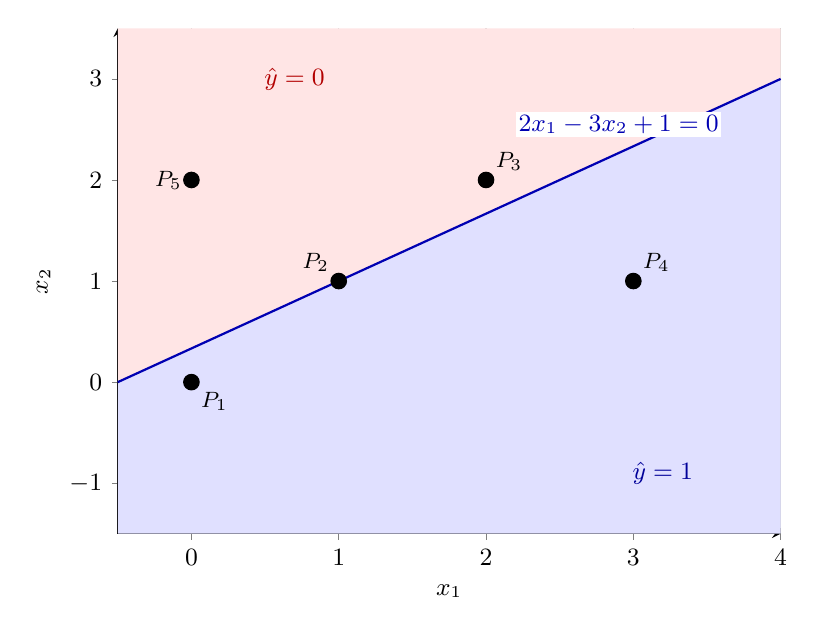
\begin{tikzpicture}
\begin{axis}[
    width=10cm,
    height=8cm,
    xmin=-0.5, xmax=4,
    ymin=-1.5, ymax=3.5,
    xlabel={$x_1$},
    ylabel={$x_2$},
    axis lines=left,
    enlargelimits=false,
    grid=both,
    minor tick num=0,
    grid style={line width=0.3pt, draw=gray!25},
    major grid style={line width=0.5pt, draw=gray!45},
    xtick={0,1,2,3,4},
    ytick={-1,0,1,2,3},
    tick label style={font=\small},
    label style={font=\small},
    clip=false
]

% --- lower region: \hat y = 1 ---
\addplot[
    draw=none,
    fill=blue!12
] coordinates {
    (-0.5,-1.5)
    (4,-1.5)
    (4,3)
    (-0.5,0)
} \closedcycle;

% --- upper region: \hat y = 0 ---
\addplot[
    draw=none,
    fill=red!10
] coordinates {
    (-0.5,0)
    (4,3)
    (4,3.5)
    (-0.5,3.5)
} \closedcycle;

% --- decision boundary ---
\addplot[
    thick,
    blue!70!black,
    domain=-0.5:4,
    samples=2
] {2/3*x + 1/3};

% --- boundary annotation ---
\node[
    font=\small,
    blue!70!black,
    fill=white,
    inner sep=1pt
] at (axis cs:2.9,2.55) {$2x_1-3x_2+1=0$};

% --- region labels ---
\node[
    font=\small\bfseries,
    text=blue!60!black
] at (axis cs:3.2,-0.9) {$\hat y=1$};

\node[
    font=\small\bfseries,
    text=red!70!black
] at (axis cs:0.7,3.0) {$\hat y=0$};

% --- sample points ---
\addplot[
    only marks,
    mark=*,
    mark size=2.8pt,
    black
] coordinates {
    (0,0)
    (1,1)
    (2,2)
    (3,1)
    (0,2)
};

% --- point labels ---
\node[font=\footnotesize, below right] at (axis cs:0,0) {$P_1$};
\node[font=\footnotesize, above left]  at (axis cs:1,1) {$P_2$};
\node[font=\footnotesize, above right] at (axis cs:2,2) {$P_3$};
\node[font=\footnotesize, above right] at (axis cs:3,1) {$P_4$};
\node[font=\footnotesize, left]        at (axis cs:0,2) {$P_5$};

\end{axis}
\end{tikzpicture}
\end{center}

\subsection*{Question 3 — Classification of points}

\begin{center}
\renewcommand{\arraystretch}{1.5}
\begin{tabular}{ccccc}
\toprule
Point & $x_1$ & $x_2$ & $z = 2x_1 - 3x_2 + 1$ & $\hat{y}$ \\
\midrule
$P_1$ & 0 & 0 & $1$  & 1 \\
$P_2$ & 1 & 1 & $0$  & 1 \\
$P_3$ & 2 & 2 & $-1$ & 0 \\
$P_4$ & 3 & 1 & $4$  & 1 \\
$P_5$ & 0 & 2 & $-5$ & 0 \\
\bottomrule
\end{tabular}
\end{center}

\subsection*{Question 4 — Adjusting the bias for $Q=(1,2)$}

First, check the current classification of $Q$:
\[
  z_Q = 2(1) - 3(2) + 1 = 2 - 6 + 1 = -3 < 0 \;\Rightarrow\; \hat{y} = 0.
\]
$Q$ is currently in class 0. We want $\hat{y}=1$, i.e.\ $z_Q \geq 0$:
\[
  2(1) - 3(2) + b \geq 0 \;\Rightarrow\; -4 + b \geq 0 \;\Rightarrow\; b \geq 4.
\]

\begin{tcolorbox}[answerbox, title={Answer}]
Any bias $b \geq 4$ classifies $Q=(1,2)$ as class~1 while keeping $w_1=2$, $w_2=-3$ unchanged.
The minimal change is $b = 4$ (the boundary passes exactly through $Q$).

\textbf{Note:} increasing $b$ shifts the boundary line upward ($x_2 = \tfrac{2}{3}x_1 + \tfrac{b}{3}$),
enlarging the region classified as~1.
\end{tcolorbox}

% =============================================================
\section{Forward Propagation in a 2-2-1 MLP}
% =============================================================

\subsection*{Question 1 — Complete forward pass}

We compute $z_i^{(1)} = \sum_j W^{(1)}_{ij} x_j + b^{(1)}_i$ then $h_i = f(z_i^{(1)})$, then
$z^{(2)} = W^{(2)\top} h + b^{(2)}$ and $\hat{y} = f(z^{(2)})$.

\vspace{0.8em}

\textbf{Input $(0, 0)$:}
\[
  z_1^{(1)} = 1\cdot0 + 1\cdot0 - 1.5 = -1.5 \;\Rightarrow\; h_1 = 0
\]
\[
  z_2^{(1)} = 1\cdot0 + (-1)\cdot0 - 0.5 = -0.5 \;\Rightarrow\; h_2 = 0
\]
\[
  z^{(2)} = 1\cdot0 + 1\cdot0 - 1.5 = -1.5 \;\Rightarrow\; \hat{y} = 0
\]

\textbf{Input $(0, 1)$:}
\[
  z_1^{(1)} = 0 + 1 - 1.5 = -0.5 \;\Rightarrow\; h_1 = 0
\]
\[
  z_2^{(1)} = 0 - 1 - 0.5 = -1.5 \;\Rightarrow\; h_2 = 0
\]
\[
  z^{(2)} = 0 + 0 - 1.5 = -1.5 \;\Rightarrow\; \hat{y} = 0
\]

\textbf{Input $(1, 0)$:}
\[
  z_1^{(1)} = 1 + 0 - 1.5 = -0.5 \;\Rightarrow\; h_1 = 0
\]
\[
  z_2^{(1)} = 1 + 0 - 0.5 = 0.5 \;\Rightarrow\; h_2 = 1
\]
\[
  z^{(2)} = 0 + 1 - 1.5 = -0.5 \;\Rightarrow\; \hat{y} = 0
\]

\textbf{Input $(1, 1)$:}
\[
  z_1^{(1)} = 1 + 1 - 1.5 = 0.5 \;\Rightarrow\; h_1 = 1
\]
\[
  z_2^{(1)} = 1 - 1 - 0.5 = -0.5 \;\Rightarrow\; h_2 = 0
\]
\[
  z^{(2)} = 1 + 0 - 1.5 = -0.5 \;\Rightarrow\; \hat{y} = 0
\]

\vspace{0.5em}

\textbf{Summary table:}

\begin{center}
\renewcommand{\arraystretch}{1.6}
\begin{tabular}{cc|cc|cc|cc}
\toprule
$x_1$ & $x_2$ & $z_1^{(1)}$ & $h_1$ & $z_2^{(1)}$ & $h_2$ & $z^{(2)}$ & $\hat{y}$ \\
\midrule
0 & 0 & $-1.5$ & 0 & $-0.5$ & 0 & $-1.5$ & \textbf{0} \\
0 & 1 & $-0.5$ & 0 & $-1.5$ & 0 & $-1.5$ & \textbf{0} \\
1 & 0 & $-0.5$ & 0 & $\phantom{-}0.5$ & 1 & $-0.5$ & \textbf{0} \\
1 & 1 & $\phantom{-}0.5$ & 1 & $-0.5$ & 0 & $-0.5$ & \textbf{0} \\
\bottomrule
\end{tabular}
\end{center}

\subsection*{Question 2 — Logical function}

\begin{tcolorbox}[answerbox, title={Answer}]
The output is always $\hat{y} = 0$: this network does \textbf{not} implement any useful logical
function as configured. It is equivalent to the \emph{constant zero} function.

\medskip
\textbf{Why?} The output neuron fires only if $h_1 + h_2 \geq 1.5$, i.e.\ only when
\emph{both} $h_1 = 1$ \emph{and} $h_2 = 1$ simultaneously. But $h_1 = 1$ requires
$x_1 + x_2 \geq 1.5$ (both inputs at least partially active), while $h_2 = 1$ requires
$x_1 - x_2 \geq 0.5$ (i.e.\ $x_1$ strictly larger than $x_2$). No binary input pair
satisfies both conditions at once.

\medskip
\textbf{Remark for students:} this illustrates how weight choice is critical.
Because $W^{(2)} = (1,\,1)^\top$, the output neuron cannot distinguish which hidden neuron
fired: it sees only $h_1 + h_2$. Since $h_1$ and $h_2$ never fire simultaneously on binary
inputs (as shown above), $h_1 + h_2 \in \{0, 1\}$ for all inputs, and no value of $b^{(2)}$
alone can separate $(1,1)$ from $(1,0)$.

To implement AND, one must also change the output weights. For instance, setting
$W^{(2)} = (1,\,0)^\top$ and $b^{(2)} = -0.5$ gives $\hat{y} = f(h_1 - 0.5)$,
which fires exactly when $h_1 = 1$, i.e.\ only for the input $(1,1)$ --- correctly
implementing AND.

Alternatively, setting $W^{(1)}_{2,\cdot} = (1, 1)$ with $b^{(1)}_2 = -0.5$ (so $h_2$
becomes a copy of $h_1$ shifted by a different threshold) and keeping $W^{(2)} = (1,1)^\top$
with $b^{(2)} = -1.5$ would also work, since both $h_1$ and $h_2$ would then fire together.
\end{tcolorbox}

\subsection*{Question 3 — Geometric interpretation of hidden neurons}

\textbf{Hidden neuron $h_1$} fires when $z_1^{(1)} \geq 0$:
\[
  x_1 + x_2 - 1.5 \geq 0 \;\Longleftrightarrow\; x_1 + x_2 \geq 1.5.
\]
This is the half-plane \emph{above} the diagonal line $x_1 + x_2 = 1.5$.
It only activates when both inputs are simultaneously large.

\vspace{0.5em}

\textbf{Hidden neuron $h_2$} fires when $z_2^{(1)} \geq 0$:
\[
  x_1 - x_2 - 0.5 \geq 0 \;\Longleftrightarrow\; x_1 - x_2 \geq 0.5.
\]
This is the half-plane \emph{below} the line $x_2 = x_1 - 0.5$, i.e.\ where $x_1$
is significantly larger than $x_2$.

\begin{tcolorbox}[solutionbox]
Each hidden neuron defines a \textbf{linear boundary} in the input plane:
\[
  h_1: \quad x_1 + x_2 = 1.5
  \qquad\qquad
  h_2: \quad x_1 - x_2 = 0.5
\]
These two lines partition the plane into regions. The output layer then combines
these two binary detectors --- illustrating how an MLP builds complex regions by
intersecting the half-planes of its hidden neurons.
\end{tcolorbox}

% =============================================================
\section{Designing MLP Architectures}
% =============================================================

\subsection*{Task A — Spam Detection}

\textbf{a) Proposed architecture:} $20 \to 16 \to 1$
\begin{itemize}[itemsep=0.2em]
  \item Input layer: 20 neurons (one per feature).
  \item Hidden layer: 16 neurons with ReLU activation.
  \item Output layer: 1 neuron with \textbf{sigmoid} activation (binary probability).
\end{itemize}

\textbf{b) Parameter count:}
\[
  \underbrace{(20 \times 16) + 16}_{\text{input} \to \text{hidden}} +
  \underbrace{(16 \times 1) + 1}_{\text{hidden} \to \text{output}}
  = 320 + 16 + 16 + 1 = \mathbf{353} \text{ parameters.}
\]

\begin{tcolorbox}[answerbox, title={Note on architecture choices}]
Any reasonable hidden layer size (e.g.\ 8, 16, 32 neurons) is acceptable.
The key constraints are: \textbf{20 input neurons}, \textbf{1 output neuron with sigmoid}.
The sigmoid maps the output to $[0,1]$, interpreted as $P(\text{spam})$.
\end{tcolorbox}

\subsection*{Task B — Handwritten Digit Recognition}

\textbf{a) Number of inputs:}
\[
  28 \times 28 = \mathbf{784} \text{ input neurons (one per pixel).}
\]

\textbf{b) Output layer:} \textbf{10 neurons} (one per digit class, 0--9) with
\textbf{softmax} activation, so that outputs sum to 1 and can be interpreted as class
probabilities.

\textbf{c) Architecture $784 \to 128 \to 10$ — parameter count:}
\[
  \underbrace{(784 \times 128) + 128}_{\text{input} \to \text{hidden}} +
  \underbrace{(128 \times 10) + 10}_{\text{hidden} \to \text{output}}
  = 100352 + 128 + 1280 + 10 = \mathbf{101\,770} \text{ parameters.}
\]

\subsection*{Task C — Open Question}

\textbf{a) Parameter count for $784 \to 10 \to 10$:}
\[
  \underbrace{(784 \times 10) + 10}_{\text{input} \to \text{hidden}} +
  \underbrace{(10 \times 10) + 10}_{\text{hidden} \to \text{output}}
  = 7840 + 10 + 100 + 10 = \mathbf{7\,960} \text{ parameters.}
\]

\textbf{b) Critical analysis:}

\begin{tcolorbox}[solutionbox]
This architecture is \textbf{almost certainly too small} for handwritten digit recognition.

The hidden layer has only 10 neurons, creating an \emph{information bottleneck}: the network
must compress the 784-dimensional input into just 10 intermediate values before making a
decision. In practice, networks of this size learn poorly because they lack the capacity to
represent the variety of handwriting styles.

For reference, a single hidden layer of 128 neurons (Task B) already reaches $\sim$97\%
accuracy on MNIST with standard training. The student's architecture has $\sim$13$\times$
fewer parameters in the hidden layer, which strongly limits expressiveness. This illustrates
that \textbf{model capacity must match task complexity}: too few neurons leads to
underfitting.
\end{tcolorbox}

\end{document}
